\chapter{SED \textit{\&} SED Modelling}\label{chp:SED}
\captionsetup{width=0.75\textwidth}

Galaxies emit radiation over the full electromagnetic spectrum, due to contributions from various components, including stars, gas, dust, and active galactic nuclei (AGN). A galaxy's Spectral Energy Distribution (SED) refers to the distribution of its emitted light across different wavelengths or frequencies.

%-------------------------------------------------------------------------------%
%-------------------------------------------------------------------------------%
%-------------------------------------------------------------------------------%
%-------------------------------------------------------------------------------%
%-------------------------------------------------------------------------------%
\section{Spectral Energy Distribution of Galaxies} \label{sec:SED}

Spectral Energy Distributions (SEDs) are discretely sampled functions of energy that describe the luminous output of an astronomical object. The independent variable is the photon energy of radiation, more often represented by frequency or wavelength. The dependent variable is the energy flux from the object which is the energy received from the source on the surface of the Earth assuming that is free of atmospheric or local absorption effects. This measurement is usually represented in energy units such as erg/s or Watts. Observed SEDs are usually cast in luminance units (e.g., $\mbox{erg/s/cm}^2$ or $\mbox{Watt/m}^2$), and often in specific flux units (e.g., $\mbox{erg/s/cm}^2\mbox{/μm}$ or $\mbox{ Watt/m}^2\mbox{/Hz}$).\\
The Spectral Energy Distribution provides a comprehensive view of a galaxy's emission, ranging from low-energy radio waves to high-energy gamma rays, as demonstrated in Figure \ref{fig:SEDgeneral}, and, when measured with sufficient precision and suitably analysed, offers insights about a galaxy’s composition from its birth to its time of observation\cite{Acquaviva2011}.
Galaxies' SEDs can be assembled through spectrography, or constructed from the photometry of multiple surveys\cite{Walcher2011}.\\
The SED of a galaxy is shaped by stellar populations, the interstellar medium (ISM), AGN torus, emission related to accretion processes such as the accretion disk, hot corona and emission from relativistic jets. In general, galaxies emit most of their energy in the form of starlight, with the dominant contribution coming from stars across different ages and masses, diffuse dust can absorb and re-emit starlight at longer wavelengths, leading to characteristic features in the infrared. However, other components can significantly affect the SED. For example, AGN, powered by accretion onto supermassive black holes at the galaxy's center, can contribute additional energy in the form of high-energy radiation, and are the dominant component for quasars. Therefore, the main aim of SED analysis is to use an observed SED to identify and constrain the contributions from these different components.\\
By studying the SED of galaxies across different wavelengths, insights into their physical properties, evolution, and formation mechanisms can be gained. Analyzing the SEDs of large samples of galaxies helps to build a comprehensive picture of the universe's structure and history.

%https://github.com/vikalibrate/FortesFit/blob/master/docs/introduction.rst

\begin{figure}
  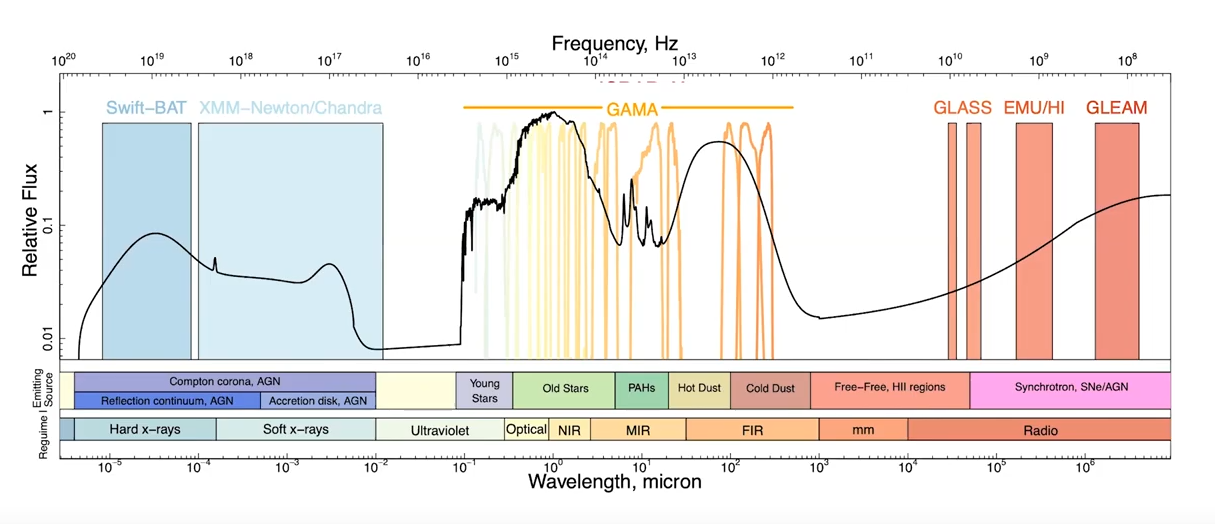
\includegraphics[width =\textwidth]{figures/SEDgeneral.png}
  \caption{An example of a panchromatic galaxy SED. Signature band-passes are plotted in color accompanied by the name of the survey where they were used. Spectral regions and related dominant component are denoted at the bottom. Image credit: Luke J. M. Davies. }
  \label{fig:SEDgeneral}
\end{figure}


\begin{figure}
  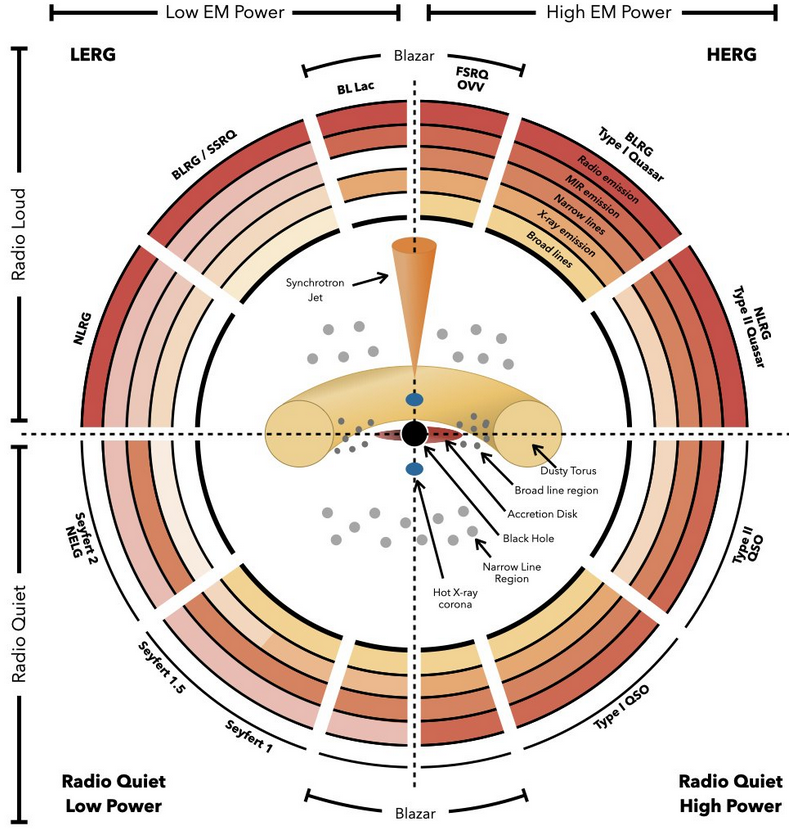
\includegraphics[width = \textwidth]{figures/UnificationThorne.png}
  \caption{Schematic representation of the AGN unified model, where the accretion disk, the torus and the relativistic jet are depicted, as well as the radio loud types of sources (in the upper part of the diagram), such as those that populate the ARC survey. The type of AGN depends on the viewing angle, whether or not the AGN produces a significant jet emission, and how powerful the central engine is. Image credit: Jessica E. Thorne. }
  \label{fig:AGNUni}
\end{figure}



%-------------------------------------------------------------------------------%
%-------------------------------------------------------------------------------%
%-------------------------------------------------------------------------------%
%-------------------------------------------------------------------------------%
%-------------------------------------------------------------------------------%

\section{Modeling the SED of galaxies} \label{sec:SEDmodelling}

\subsection{AGN Component}
Radio sources, such as those in the ARC survey, owe their synchrotron radio emission to their radio loud AGN. Radio loud sources can be categorised, as depicted in Figure \ref{fig:AGNUni}:
\begin{itemize}
    \item Radio galaxies in which the central region is hidden but show bright radio jets and large radio luminosities. They can be divided in two groups according to their radio morphology and luminosity: the low-luminosity Fanaroff-Riley class I (FR-I) and the high-luminosity Fanaroff-Riley class II (FR-II). The FR-I galaxies show compact radio emission and their radio surface brightness profiles decrease outwards, while FR-II galaxies are dominated by radio lobes and their radio surface brightness profiles increase outwards as they reach the end of the extended structures.
    \item Radio loud Quasars,which  were the first quasars to be discovered due to their strong radio emission. Their optical spectrum is similar to those of Seyfert galaxies and are therefore divided into type 1 and type 2.
    \item Radio loud Blazars, which are a special subclass of quasars, in which a relativistic jet is pointing very close to the line of sight of the observer. They have high variability and emit from radio frequencies to very high energies. 
\end{itemize}
There is great variety of AGN types and to explain this diversity Antonucci
(1993)\cite{Antonucci1993} proposed the first unification model, allowing the distinction
between Seyferts and quasars and explaining other observational differences by orientation effects. Urry and Padovani (1995)\cite{UrryPado1995} extended the unification model by including the relativistic jet. Figure \ref{fig:AGNUni} represents the AGN unified model, with the principal components and the type of AGN depending on the viewing angle. 


\subsection{Galaxy Component}
Apart from the AGN, the host galaxy consists of the Interstellar Medium (ISM) and stars spanning a variety of spectral types\cite{Conroy2013}. The Interstellar Medium contains dust\cite{ISMDust2005}\cite{ISMDust2020} and gas\cite{ISM2022}, at different phases, temperatures, densities and ionisation states. Emission from gas imprints the spectral emission lines to the full galactic spectrum, but its contribution to the SED continuum is negligible. Since the main focus of the present work is based on broad band photometric SED data, the important galaxy components shaping a galaxy's SED are considered to be the stellar content of a galaxy and the diffuse ISM dust. 


\section{Dust in the ISM} \label{sec:SED/ISMdust}
Astrophysical dust is one of the key components of the diffuse interstellar medium of galaxies.
Dust particles (“grains”) originate as a product of stellar evolution. Grains form in the atmospheres of evolved stars or remnants of supernovae, and are then released or ejected into the ISM, their sizes vary from larger than $\sim 0.02 \, $μm to nano-particle size. A robust model of dust in the diffuse ISM is proposed by Hensley \& Draine (2023)\cite{HenDraine2023}. Both extinction and emission from interstellar dust are observed. Observationally, the presence of dust in galaxies is revealed by two general effects: 
\begin{itemize}
    \item dust produces emission in the infrared (IR) part of the spectrum, consisting of the dust continuum emission spectrum and various emission and absorption features
    \item dust modifies the light that originates from the stellar continuum at all wavelengths, in particular the ultraviolet (UV) to near-infrared (NIR) flux from stars is attenuated by dust
\end{itemize}

\subsection{Dust extinction}\label{sec:DustExt}
Extinction represents the amount of light lost along a single line of sight through a dusty medium due to absorption or scattering away from the line of sight. The total extinction $\tau_\lambda$ per hydrogen column density $N_H$ at wavelength $\lambda$ for a population of randomly oriented grains is:
\begin{equation}
    \dfrac{\tau_\lambda}{N_H} = \sum_{i=1}^N \, \int \,da\,\Big(\frac{1}{n_H}\dfrac{dn_i}{da} \Big) \,C^{\text{\tiny{ext}}}_{\text{\tiny{ran}}}(\lambda, i, a) \label{eq:extiction}
\end{equation}
where $N$ is the number of distinct components in the model, each grain component $i$ in the model has a size distribution $dn_i /da$ defined such that the number density of grains having an effective radius between $a$ and $a + da$ is $(dn_i/da) da$, $C^{\text{\tiny{ext}}}_{\text{\tiny{ran}}}$ denotes the extinction cross section for randomly oriented grains.\\
\begin{figure}
\centering
  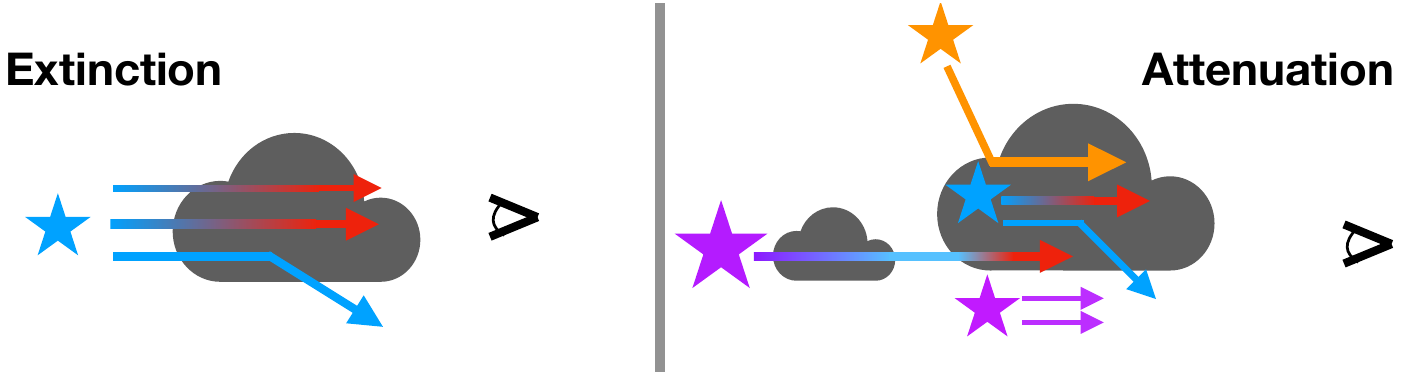
\includegraphics[width = 0.8 \textwidth]{figures/SalimDust.png}
 \caption{Difference between dust extinction and dust absorption of stellar light. Image lifted from Salim \& Narayanan (2020)\cite{SalimNara2020}. }
  \label{fig:Dust_extatt}
\end{figure}
As described in detail by Salim \& Narayanan (2020)\cite{SalimNara2020}, in contrast to extinction, attenuation includes the effects arising from the distribution of stars and dust in the galaxy,. Attenuation includes the same mechanisms for loss of photons as extinction plus scattering back into the line of sight, as well as the contribution to the light by unobscured stars, schematically shown in Figure \ref{fig:Dust_extatt}. 
In panel (e) of Figure \ref{fig:SSP_all} the radiative transfer based attenuation curve of Witt \& Gordon (2000)\cite{WittGord2000} is shown in dashed lines, along with the average attenuation model of Calzetti (2000)\cite{Calzetti2000} for star-forming galaxies. The evidence-based average attenuation law of Calzetti (2000)\cite{Calzetti2000} proposes that the observed flux from stars in the presence of dust is
\begin{equation}
    F_{\mbox{\tiny{obs}}}(\lambda) = F_{\mbox{\tiny{intr}}}(\lambda) \times 10^{-0.4 \, A_{\lambda}} \label{eq:dustatten} 
\end{equation}
where $F_{\mbox{\tiny{obs}}}(\lambda)$ is the observed (attenuated) stellar flux, $F_{\mbox{\tiny{intr}}}(\lambda)$ is the intrinsic (unattenuated) stellar flux and the attenuation $A_\lambda$ is related to the UV-visual color excess E(B-V):
\begin{equation}
    A_{\lambda} = k(\lambda)\, \mbox{E(B-V)} \label{eq:dustatten2} 
\end{equation}
and the absorption coefficient $k(\lambda)$ follows:
\begin{equation}
     k(\lambda)  = \begin{cases} R_{\nu} + 2.659 \times \Big( -2.156 + \dfrac{1.509}{\lambda} - \dfrac{0.198}{\lambda^2} + \dfrac{0.011}{\lambda^3}  \Big) \;\;\;\; ,\;0.12 \,μm \leq \lambda \leq 0.63 \, μm
    \\  \\ R_{\nu} +2.659 \times \Big( -1.857 + \dfrac{1.040}{\lambda}\Big) \;\;\;\;\;\;\;\;\;\;\;\;\;\;\;\; ,\;0.63 \,μm \leq \lambda \leq 2.2 \, μm \end{cases} \label{eq:dustatten3} 
\end{equation}
with $R_{\nu} = 4.05$ and the coefficients adjusted for $\lambda$ in microns.


\subsection{Dust emission}
There are two principal emission mechanisms for interstellar grains: thermal vibrational emission $I^{\text{\tiny{th}}}_\lambda$ and rotational emission $I^{\text{\tiny{SpD}}}_\lambda$ (“spinning dust emission”). The total dust emission per hydrogen atom $I_\lambda /N_H$ is the sum of these two contributions\cite{HenDraine2023}:
\begin{equation}
    \dfrac{I_\lambda}{N_H} = \dfrac{I^{\text{\tiny{th}}}_\lambda}{N_H}  + \dfrac{I^{\text{\tiny{SpD}}}}{N_H}  
\end{equation}
Interstellar grains absorb UV and optical starlight and reradiate the energy in the infrared, the resulting thermal vibrational emission per $N_H$ from a population of randomly oriented dust grains is:
\begin{equation}
    \dfrac{I^{\text{\tiny{th}}}_\lambda}{N_H} =  \sum_{i=1}^N \, \int \,da\,\Big(\frac{1}{n_H}\dfrac{dn_i}{da} \Big) \times \int \,dT\, \Big( \dfrac{dP}{dT}\Big)_{i,a}\,C^{\text{\tiny{abs}}}_{\text{\tiny{ran}}}(\lambda, i, a) \, B_\lambda(T)
\end{equation}
where $B_\lambda(T)$ is the Planck function and $(dP/dT )_{i,a}$ is the grain temperature distribution of grains of composition $i$ and effective radius $a$. Contribution from stimulated emission is negligible in radiation fields typical of the diffuse ISM and, thus, ignored. Assuming\cite{HenDraine2023} a radiation field with specific energy density $u_\lambda$: 
\begin{equation}
    u_\lambda = U \, \Big[ u^{\text{\tiny{UV}}}_\lambda   + \sum_{i=1}^{3} \dfrac{4\pi}{c} W_i B_\lambda(T_i)\Big] + \dfrac{4\pi}{c} B_\lambda(T_{\text{\tiny{CMB}}})
\end{equation}
where $U$ is a frequency independent scaling factor, $u^{\text{\tiny{UV}}}_\lambda $ is the UV component of the radiation field, and $T_{\text{\tiny{CMB}}} =2.725$ K is the CMB temperature. The optical starlight component is modeled as three black bodies having temperatures of $T_1 = 3000$ K, $T_2 = 4000$ K and $T_3 = 7500$ K with dilution factors $W_1 = 7\times10^{-13}$, $W_2 = 1.65\times10^{-13}$ and $W_3 = 10^{-14}$. The UV component is given by
\begin{equation}
     \dfrac{\lambda \, u^{\text{\tiny{UV}}}_\lambda}{\text{erg}\;\text{ cm}^{-3}}  = \begin{cases} 2.373 \times10^{-14}\; (\frac{\lambda}{\mu \text{m}})^{-0.6678} \;\;\;\;\;\; ,\;1340\,\textup{~\AA} <\lambda < 2460\,\textup{~\AA}
    \\  6.825 \times10^{-13}\; (\frac{\lambda}{\mu \text{m}})\;\;\;  \;\;\;\;\;\;\;\;\;\;\;\;,\; 1100\,\textup{~\AA} <\lambda < 1340\,\textup{~\AA}\\ 1.287 \times10^{-13}\; (\frac{\lambda}{\mu \text{m}})^{4.4172} \;\;\;\;\;\;\;\;\;  ,\;912\,\textup{~\AA} <\lambda < 1100\,\textup{~\AA}\\ 0 \;\;\;\;\;\;\;\;\;\;\;\;\;\;\;\;\;\;\;\;\;\;\;\;\;\;\;\;\;\;\;\;\;\;\;\;\;\;\;\;\; ,\;    \lambda <912 \,\textup{~\AA} \end{cases}
\end{equation}
Stimulated IR emission from the dust itself does not appreciably contribute to the heating of dust grains in radiation fields typical of the diffuse ISM and is, thus, neglected.\\
To ensure consistency between the power absorbed by dust (having the adopted extinction curve \ref{eq:extiction}) and the power emitted by dust, it is required that $\log_{10} U \approx 0.2$ (yielding $U \approx 1.6$). Several factors contribute to the larger value of $U$ and introduce constraints on IR emission and differences in the dust model.\\
It is remarked by Hensley \& Draine (2023)\cite{HenDraine2023} that in addition to thermal vibrational emission, rapidly rotating ultra small grains can also produce electric or magnetic dipole emission. This mechanism has been identified peaking near 30 GHz and is dependent on environmental parameters.
%The mid-infrared (MIR) spectral band 

\subsection{Dust model \textit{\&} parameters}
Joint AGN and star-forming SED models for dust emission are presented by Dale et al. (2014)\cite{Dale2014}. The dust emission templates for the star-forming component are used in the present code, available from Daniel Dale\footnote{\url{http://physics.uwyo.edu/~ddale/research/seds/seds.html}}.
In the construction of the templates, a series of “local” spectral energy distributions were created to represent the emission from dust exposed to a wide range of heating intensities $0.3 \leq U \leq 10^5$ where $U = 1$ corresponds to the local interstellar radiation field in the Solar Neighborhood. A power-law combination of these local curves can effectively mimic the spatially-integrated (“global”) dust emission:
\begin{equation}
     dM_d \propto U^{-\alpha_{\text{\tiny{SF}}}}\,dU
\end{equation}
where $M_d$ is the dust mass heated by a radiation field at intensity $U$ and the exponent $\alpha_{\text{\tiny{SF}}}$ represents the relative contributions of the different local spectral energy distributions. A single parametre ($\alpha_{\text{\tiny{SF}}}$) is used to describe the full range of PAH/very small grain/large grain and overall spectral shapes for normal star-forming galaxies. 
The star-forming dust emission templates are based on spectral shapes of starburst galaxies from the Spitzer archives and include prominent fine-structure lines such as [Ne III]15.6 μm, [S III]18.7 μm, and [S III]33.5 μm and the 17 μm PAH complex, the latter of which accounts for up to 10\% of the total PAH emission in normal star-forming galaxies. \\
The Dale et al. (2014)\cite{Dale2014} ISM dust models for star-forming galaxies are used in the present work, parametrised with the exponential $\alpha_{\text{\tiny{SF}}}$ and the number of atoms (which contribute to the dust mass), in Figure \ref{fig:Dust_temp} the templates are shown for different values of $\alpha_{\text{\tiny{SF}}}$, while the number of particles is a scaling factor.
\begin{figure}
  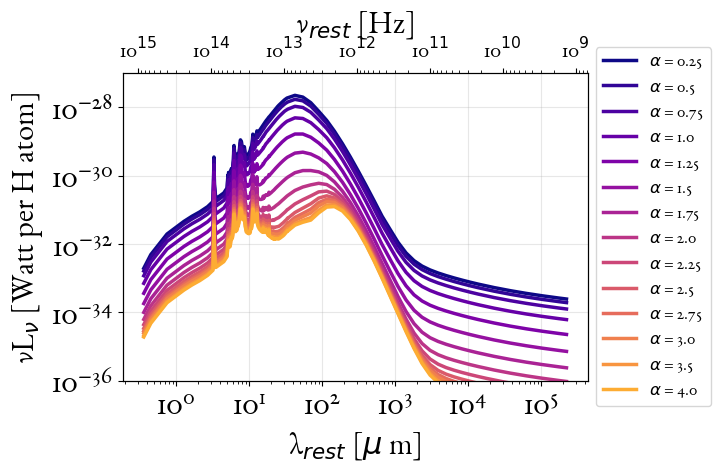
\includegraphics[width = \textwidth]{figures/Templates/Dust_ISM.png}
 \caption{ISM dust emission Dale et al. (2014)\cite{Dale2014} for different values of $\alpha_{\text{\tiny{SF}}}$. }
  \label{fig:Dust_temp}
\end{figure}
The models are given in units of Watt and are normalised to the emission from a particle with mass equal to single hydrogen atom. For ease of use in the present work, the intensity has been transformed to erg/s and the normalisation has been converted to the luminosity of one solar mass ($M_\odot$).

%-------------------------------------------------------------------------------%
%-------------------------------------------------------------------------------%
%-------------------------------------------------------------------------------%
%-------------------------------------------------------------------------------%
%-------------------------------------------------------------------------------%
\section{Stellar Populations} \label{sec:SED/Stellar}

The visible and near-infrared (NIR) spectral windows on a galaxy's SED are dominated by the radiation of the stars on the galaxy. \\
The stellar populations of a galaxy have a range of luminosities, masses, ages and metallicities with some being present from when the galaxy first formed and other being formed more recently. Stellar Population Synthesis (SPS) is a method developed for constructing a galactic spectrum from the sum of the spectra of its stars and rely on stellar evolution theory to constrain the range of possible stellar types at a given age and metallicity. Commonly, SPS models start with a Simple Stellar Population (SSP), integrated along the evolutionary track.

\subsection{Simple Stellar Population}
A Single Stellar Population is the spectrum of an ideal, coeval ensemble of stars at a single metallicity and abundance pattern, based on a library of model stellar spectra. The evolution of this ensemble of stars is captured by the isochrones and its mass depends both on the initial distribution (Initial Mass Function) and the age of the ensemble. The Initial Mass Function (IMF) dictates how many stars of each spectral class exist initially, the isochrones dictate how the number of massive stars changes with time and the shape of a single star's spectrum is retrieved from the stellar spectra library.\\
The flux emitted per unit frequency $f_{\nu, \text{\tiny{SSP}}}$, of a SSP of mass $M$, age $t$, and metallicity $Z$ is given\cite{Conroy2013} by the sum of the individual stars:
\begin{equation}
    f_\nu ^{\text{\tiny{ SSP}}}(t,Z) = \int_{m_l}^{m_u(t)} \, f_\nu^{\text{\tiny{ star}}}\big(T_{\text{\tiny{eff}}} (M), \log g(M) ; t, Z \big)\, \xi(M ; t, Z) \,dM \label{eq:SSP}
\end{equation}
where $M$ is the initial (zero-age main sequence) stellar mass, $\xi(M ; t, Z)$ is the stellar mass function, which is computed from the initial mass function $\xi_o(M )$ and the stellar evolution which describes when and which stars will stop contributing to the SSP spectra because they end their lives either
as Supernovae or as white dwarfs\cite{Walcher2011}. $f_{\text{\tiny{star}}}$ is a stellar spectrum, and $f_{\text{\tiny{SSP}}}(t,Z)$ is the resulting time and metallicity-dependent SSP spectrum. The lower limit of integration, $m_l$, is typically\cite{Conroy2013} taken to by the hydrogen burning limit (either $0.08 M_\odot$ or $0.1 M_\odot$ depending on the SPS modelling), and the upper limit is dictated by stellar evolution. 
The isochrones specify the relation\cite{Conroy2013} between the effective temperature of a star $T_{\text{\tiny{eff}}}$, the measure of surface gravity $\log g$ and the mass of the star $M$ for a given age $t$ and metallicity $Z$. The creation of stellar isochrones requires\cite{Walcher2011} a large grid of evolutionary tracks, created by modelling the evolution of stars of a given initial mass and metal content. The Padova\cite{Padova1994} \cite{Padova2000} \cite{Padova2008} Stellar Isochrones for some indicative SSP ages are plotted in panel (b) of Figure \ref{fig:SSP_all}.
\begin{figure} 
\centering
  \subcaptionbox{IMFs  }{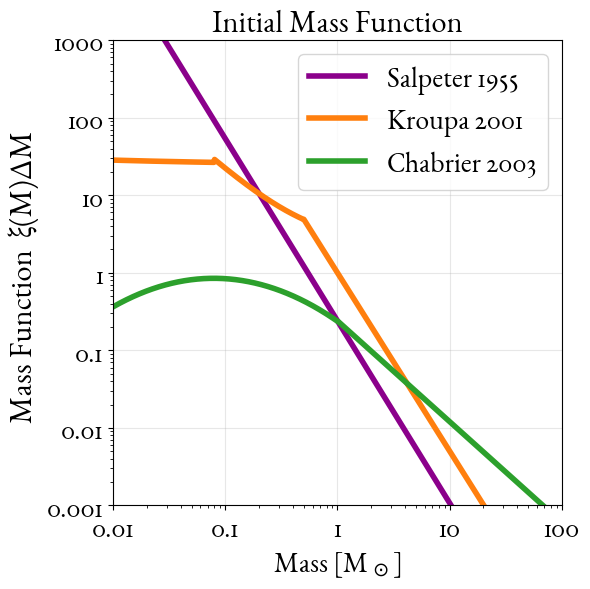
\includegraphics[width = 0.31\textwidth]{figures/Templates/IMFs_lo.png}}\quad 
  \centering
  \subcaptionbox{Stellar Isochrones }{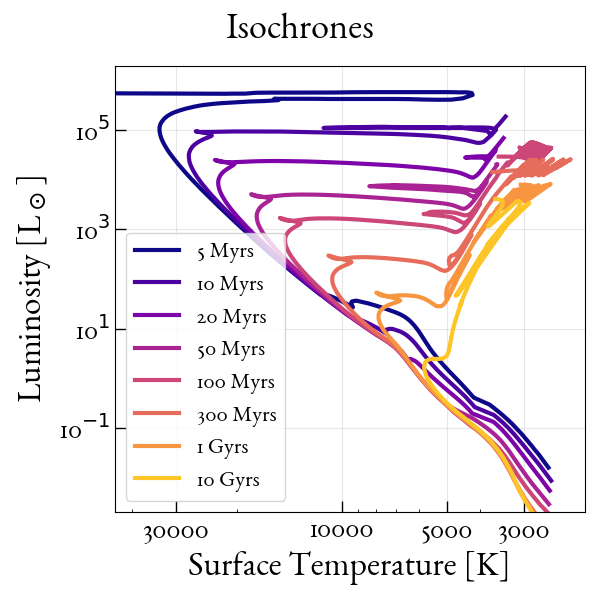
\includegraphics[width = 0.31\textwidth]{figures/Templates/isochrones_lo.png}}\quad
   \subcaptionbox{SFH }{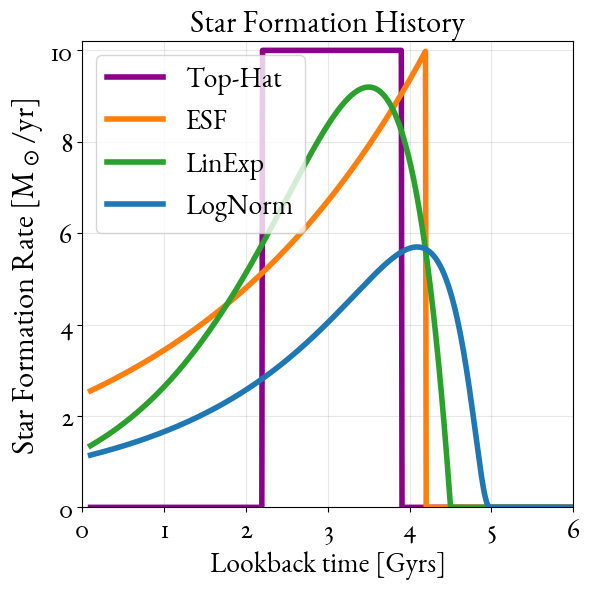
\includegraphics[width = 0.31\textwidth]{figures/Templates/SFHs.png}} \\
  
  \subcaptionbox{Model Stellar Spectra }{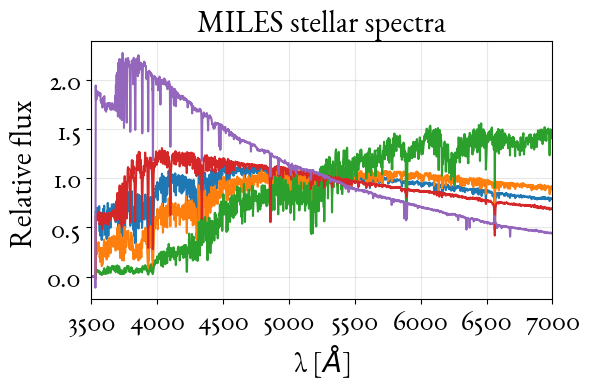
\includegraphics[width = 0.57\textwidth]{figures/Templates/MILES_T.png}} \quad 
  \subcaptionbox{Dust attenuation laws }{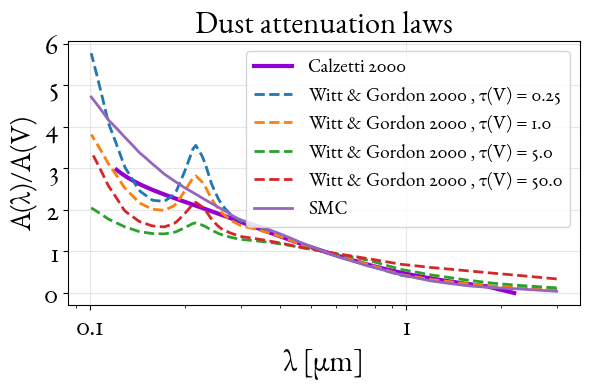
\includegraphics[width = 0.57\textwidth]{figures/Templates/DustAtt_laws.png}} 
  \caption{Panel (a): Different types of Initial Mass Functions, the model used in the present work is the Chabrier 2003\cite{Chabrier2003} Panel (b): The Padova\cite{Padova1994} \cite{Padova2000} \cite{Padova2008} Stellar Isochrones for different age of the coeval population. Panel (c): Different types of Star Formation Histories, in the present work the delayed exponential decay function is used here denoted as "LinExp". Panel (d): The empirical library of MILES model spectra \cite{MILES2}\cite{MILES2}\cite{MILES3} is used for the Stellar Population Model of the present work. Panel (e): Different Dust attenuation laws are shown. In the Stellar Population Model of this work, the Calzetti 2000\cite{Calzetti2000} law is used. }
  \label{fig:SSP_all}
\end{figure}

%--------------------------------------------------------------------------------%
%--------------------------------------------------------------------------------%
%--------------------------------------------------------------------------------%
\subsection{Stellar Evolution, Star Formation History \textit{\&} Dust Absorption}\label{sec:SFH}
The Simple Stellar Population models the flux of stars at a single specific age and metallicity. In order to represent the whole stellar population of a galaxy and combine energy and timescales of all evolutionary phases, the SSP spectrum ought to be convolved with a Star Formation History that can simulate the stellar evolution of an ensemble of stars. 
\subsubsection*{Star Formation History}
The Star Formation History is an estimate of the galaxy’s star formation rate (SFR) as a function of time, which traces its evolution and merger history\cite{Leja2013}. In Panel (c) of Figure \ref{fig:SSP_all} four common families of SFH functions are plotted:
\begin{itemize}
    \item Top-Hat, which assumes constant star formation from a start time through the time of observation at a fixed rate
    \begin{equation}
        SFR(t; t_0, \tau) = \Theta(t-t_0)\times  \Big[1- \Theta(t-t_0-\tau) \Big] \label{eq:SFHtophat}
    \end{equation}
    \item ESF assumes an exponentially declining star formation rate, and performs well for local ellipticals
    \begin{equation}
        SFR(t; t_0, \tau) = \Theta(t-t_0) \times \exp{\Big(- \dfrac{t-t_0}{\tau} \Big) }
        \label{eq:SFHesf}
    \end{equation}
    \item LinExp has a functional form of a delayed exponential decay
    \begin{equation}
        SFR(t; t_0, \tau) = \Theta(t-t_0) \times \dfrac{t-t_0}{\tau} \times\exp{\Big(- \dfrac{t-t_0}{\tau} \Big)} 
        \label{eq:SFHlinexp}
    \end{equation}
    \item LogNormal has a functional form that appears in many physical processes
    \begin{equation}
        SFR(t; t_0, \tau) = \Theta(t-t_0) \times \dfrac{1}{t} \times\exp{\big[- \dfrac{\Big(\ln(t-t_0)\big)^2}{2\tau^2} \Big]} 
        \label{eq:SFHlognorm}
    \end{equation}
\end{itemize}
In all the above functional forms, $\Theta$ is the Heaviside step function, $\tau$ is the e-folding time which delineates the evolution of Star Formation Rate (governs the "width" of the episode of star formation), $t_0$ is the age where the galaxy star formation begins, $\tau$ and $t_0$ are parametres of the functional form, while $t$ is the free variable of time.\\
For a Simple Stellar Population, which assumes that all of its stars form at a single lookback
time ($T$) and with the same metallicity ($Z$), the flux at a given frequency ($\nu$), based on equation \ref{eq:SSP}:
\begin{equation}
    f_\nu ^{\text{\tiny{ SSP}}} = \int_{0}^{t_{\mbox{\tiny{obs}}}} \, f_\nu ^{\text{\tiny{ SSP}}}(t_{\mbox{\tiny{obs}}}-t^{\prime},Z)  \; \delta(T-t_{\mbox{\tiny{obs}}}+t^{\prime}) \,dt^{\prime} 
\end{equation}
where $\delta$ is the Dirac functional, and for the lower integration limit we assume de facto that the time of the Big Bang is zero.\\
Generalising from Simple Stellar Populations (SSPs) to Composite Stellar Populations (CSPs),
we can then represent the SED for a galaxy with a given star formation history ($SFH \equiv ψ(t; t_0, \tau)$) as an integral over all star formation that occurred at different times from the
birth of the Universe to the time of observation:
\begin{equation}
    f_\nu ^{\text{\tiny{ CSP}}} = \int_{0}^{t_{\mbox{\tiny{obs}}}} \, f_\nu ^{\text{\tiny{ SSP}}}(t_{\mbox{\tiny{obs}}}-t^{\prime},Z)  \; ψ(t^{\prime}; t_0, \tau) \,dt^{\prime} \label{eq:CSP}
\end{equation}
The chosen Star Formation History in this work is the delayed exponential decay form, thus the adopted $ψ$ satisfies the constraints outlined in equation \ref{eq:SFHlinexp}:
\begin{equation*}
    ψ(t; t_0, \tau) =\Theta(t-t_0) \times \dfrac{t-t_0}{\tau} \times\exp{\Big(- \dfrac{t-t_0}{\tau} \Big)} \label{eq:SFH}
\end{equation*}
The star formation history (SFH) of a galaxy can sometimes be poorly constrained when assuming a predetermined functional form and parametrisation. And the sensitivity of model spectra to star formation drops approximately logarithmically with time, as remarked by Ocvirk et al. (2006)\cite{Ocvirk2006}.
The expanding size of galaxy catalogues available through surveys facilitates new approaches \cite{Iyer2017}\cite{Iyer2022} that aim to reconstruct the SFH from the data, using methods that include reducing the dimensionality of the parametre space using data compression methods\cite{Leja2019}, fine-binning the interval that makes the maximum contribution to flux, mapping the discretised-time photometric fitting to a linear inversion problem, or comparing against a large basis of realistic model SEDs using a Bayesian method\cite{Pacifici2013}.
 
\subsubsection*{Dust attenuation}
Dust reddening is then applied to the spectrum using the Calzetti et al. (2000)\cite{Calzetti2000} dust attenuation law as described in Section \ref{sec:DustExt}, using the E(B-V) as a free parametre of the analytical function for attenuation (equation \ref{eq:dustatten}). Thus, extending the parameter space for fitting the stellar component in the presence of dusty ISM.

\subsection{Stellar population models}

The construction of an SSP therefore requires a stellar evolution theory in the form of isochrones, stellar spectral libraries, and an IMF, each of which may. \\
In the present code Stellar Population Synthesis is not implemented directly, SPS models implemented in the code are the 2016 updated version of the Bruzual \& Charlot (2003)\cite{BC2003} models, using of the Medium-resolution Isaac Newton Telescope library of Empirical Spectra (MILES)\cite{MILES1}\cite{MILES2}\cite{MILES3}. The templates were generated using Chabrier(2003)\cite{Chabrier2003} initial mass function, spanning a range of different ages, metallicities and delayed exponential decay SFH e-folding times as depicted in Figure \ref{fig:StellarPop_temp}. The models implemented within the code are constructed using the opensource module \code{SMpy}, developed by Kenneth J. Duncan\footnote{\url{https://github.com/dunkenj/smpy}}.
In order to probe a more complex Star Formation History (Section \label{sec:SFH}), two composite stellar populations are chosen in the SED fitting code: an old stellar population and a young stellar population, each of which are parametrised by their individual stellar mass, metallicity, age, e-folding time $\tau$ and attenuation parametre (since younger stars could still reside in their birth cloud), as deposed in Table \ref{tab:ParamSpace}. The two composite stellar populations are parametrised:
\begin{itemize}
    \item Metallicity in units of solar metallicity ($Z/Z_\odot$)
    \item Age $t$ in units of Myrs
    \item E-folding time $\tau$ of delayed exponential decay SFH in units of Gyrs
    \item Stellar Mass in units of solar masses and in the logarithmic regime $\log (M_\star/M_\odot$
    \item E(B-V) extinction that couples the stellar component with the dust component via the attenuation law in functional form.
\end{itemize}
Interpolation to <0.3dex could be performed and applied in the photometric SED model, although the templates in the produced libraries, regardless of the model are fundamentally limited could not offer distinguishable SFH information for a difference smaller than 0.3-0.4 dex\cite{Ocvirk2006}. Similar-age stellar populations have very similar spectra, rendering Star Formation History recovery inherently ill-conditioned\cite{Lower2020}, as shown in Figure \ref{fig:Ocvi}.
\begin{figure}
\subcaptionbox{Composite Stellar Population with different ages }{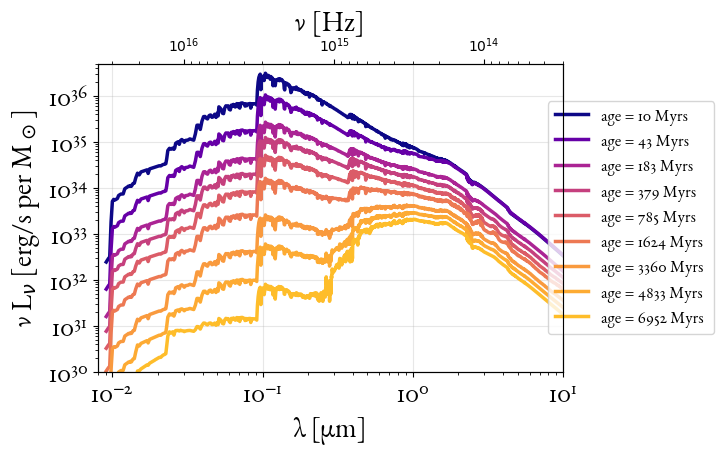
\includegraphics[width = \textwidth]{figures/Templates/SSP_T.png}}\\ 
\subcaptionbox{Composite Stellar Population with different metallicities }{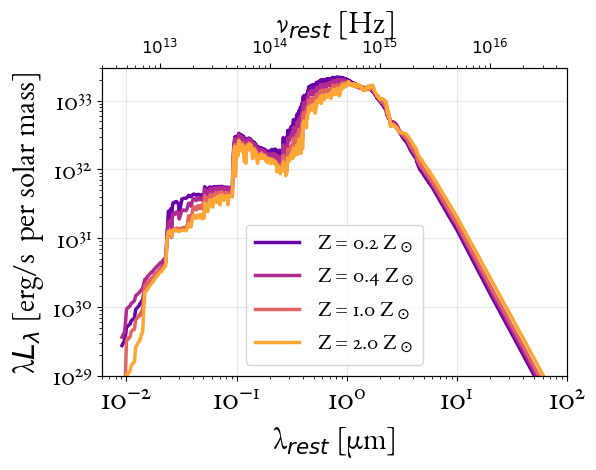
\includegraphics[width = 0.44\textwidth]{figures/Templates/Temps_Stars_metalli_oldtau2.png}} \quad \subcaptionbox{Composite Stellar Population with different e-folding time }{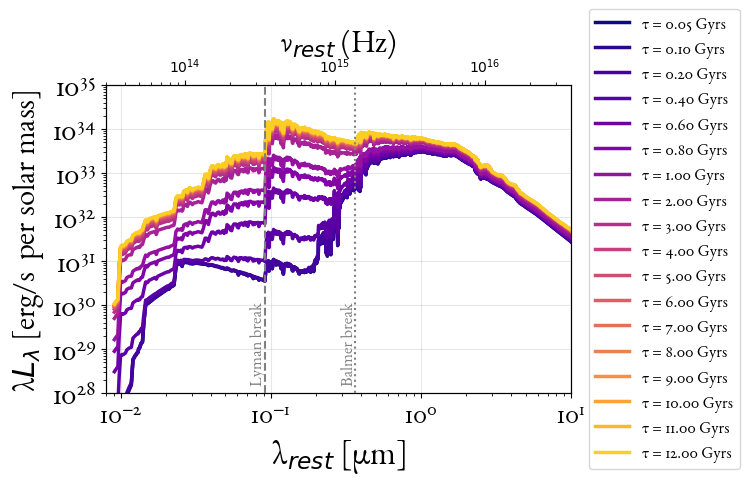
\includegraphics[width = 0.55\textwidth]{figures/Templates/Temps_Stars_tau_age3p4G.png}} 
  \caption{The Bruzual \& Charlot 2003\cite{BC2003} Stellar Population Models with the Chabrier 2003\cite{Chabrier2003} Initial Mass function, Padova\cite{Padova1994}\cite{Padova2000}\cite{Padova2008} Isochrones and a Star Formation History in the shape of delayed exponential decay, unattenuated. Panel (a): The shape changes for different age, here each spectrum has constant metallicity of $Z = Z_\odot$ and constant e-folding time of $\tau = 0.6 \; \mbox{Gyrs}$. Panel (b): The shape changes for different metallicity, here each spectrum has constant age of $10 \; \mbox{Myrs}$ and the e-folding time is $\tau = 2 \; \mbox{Gyrs}$. Panel (c): The shape changes for different e-folding time $\tau$ of the assumed Star Formation History, here each spectrum has constant age of $3.4 \; \mbox{Gyrs}$ and constant metallicity of $Z = Z_\odot$. }
  \label{fig:StellarPop_temp}
\end{figure}
\begin{figure}
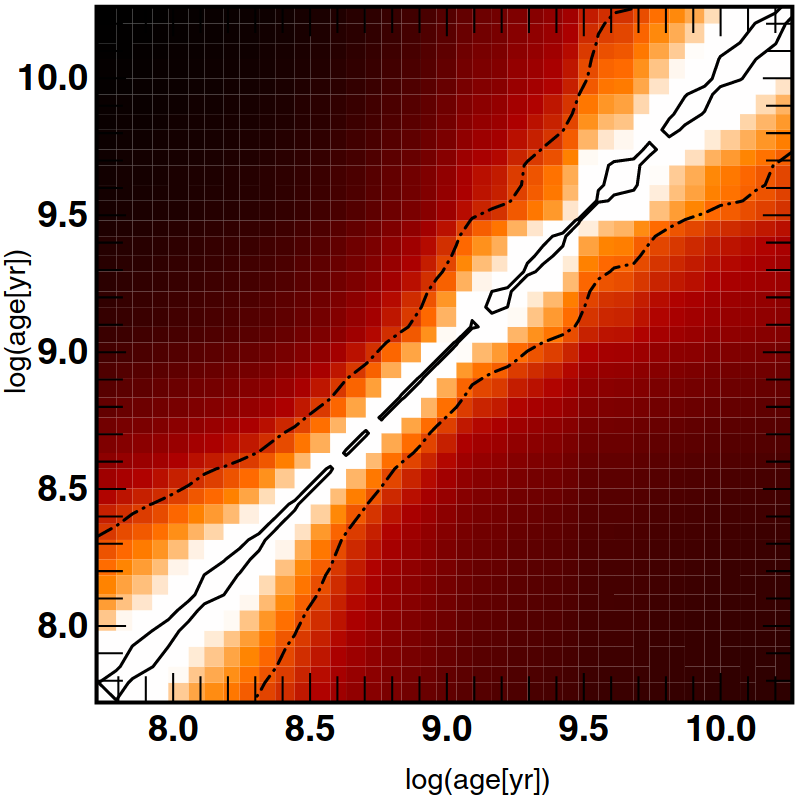
\includegraphics[width = 0.8\textwidth]{figures/Ocvirck.png}
  \caption{Distinguishability of single-age populations with Signal-to-Noise ratio S/N=10 (dash-dotted line) and with Signal-to-Noise ratio S/N=100 (continuous line). Plot lifted from Ocvirk et al. (2006)\cite{Ocvirk2006}. }
  \label{fig:Ocvi}
\end{figure}
%-------------------------------------------------------------------------------%
%-------------------------------------------------------------------------------%
%-------------------------------------------------------------------------------%
%-------------------------------------------------------------------------------%
%-------------------------------------------------------------------------------%
\section{AGN Accretion Disk}
Active galaxies host a supermassive black hole (SMBH) in their centre, which accretes the surrounding material. Because of angular momentum conservation this process leads to the formation of an accretion disk. Along with star formation, AGNs are thought to have a drastic impact on galaxy evolution. Properly disentangling the emission of AGNs from star formation is not an easy task as they can both strongly emit in the UV, and a large fraction of this emission can be reprocessed by dust and re-emitted at longer wavelengths.\\
Evidence of multiwavelength observations of quasar continua favor the geometrically thin optically thick accretion disk\cite{Malkan1983}, schematically demonstrated in Figure \ref{fig:AGNUni}. The accretion disk is made mostly out of gas and its emission is split\cite{Malkan1983} between:
\begin{itemize}
    \item Thermal emission, since particles have Maxwellian velocity distribution
due to collisions
    \item Non thermal bremmstrahlung (free-free) radiation with power-law energy distribution of particles\cite{Barvainis1993}
\end{itemize}
The accretion disk emission presents a peak in the optical spectral area, which is sometimes called Big Blue Bump (BBB). According to the virial theorem, gravitational potential energy is released half into kinetic energy and half in to radiation:
\begin{equation}
    L^{\mbox{\tiny{BBB}}} = \dfrac{ G \, \dot{M} \, M }{2\; r} \iff \dfrac{ G \; \dot{M} \; M }{2\; r} = 2 \pi r^2 \, \sigma_{\mbox{\tiny{SB}}} \, T^4 \iff T(r) = \Big(\dfrac{G \,\dot{M} \, M}{4\pi \,  \sigma_{\mbox{\tiny{SB}}} \, r^3 } \Big)^{1/4}
\end{equation}
Where, $M$ is the mass of the accreted gas, $\dot{M}$ is the accretion rate, $r$ is the distance of the accreted material from the SMBH, $\sigma_{\mbox{\tiny{SB}}}$ is the Stefan-Boltzmann constant and $G$ is the universal gravity constant.
In reality, the above is an approximation averaged over the disk, since energy is dissipated locally in the disk through viscosity. This yields:
\begin{equation}
     T(r)  = \begin{cases}   
     \Bigg[ \dfrac{3G \,\dot{M} \, M}{8\pi \,  \sigma_{\mbox{\tiny{SB}}} \, r^3 } \Big( 1- \sqrt{\dfrac{R_i}{r}}  \Big) \Bigg]^{1/4}   \;\;\; \;\;\;\;\;\;\;\;\;\;\;\;,\; r \gg R_i \\ \\ 
     \Bigg(\dfrac{3G \,\dot{M} \, M}{8\pi \,  \sigma_{\mbox{\tiny{SB}}} \, R_{\mbox{\tiny{S}}}^3 } \Bigg)^{1/4} \times \Big(  \dfrac{r}{R_{\mbox{\tiny{S}}}}  \Big)^{-1/3}  \;\;\;\;\;\;\;\;\;\;\;\;\; ,\;     r \sim R_{\mbox{\tiny{S}}} \end{cases}
\end{equation}
where $R_i$ is the inner radius of the accretion disk and $R_{\mbox{\tiny{S}}} = 2GM/c^2$ is the Schwartzschild radius. Hence, the accretion disk continuum spectrum is a superposition of many Black Bodies with different temperatures. 
\subsection{Accretion disk model \textit{\&} parametres}
\begin{figure}
  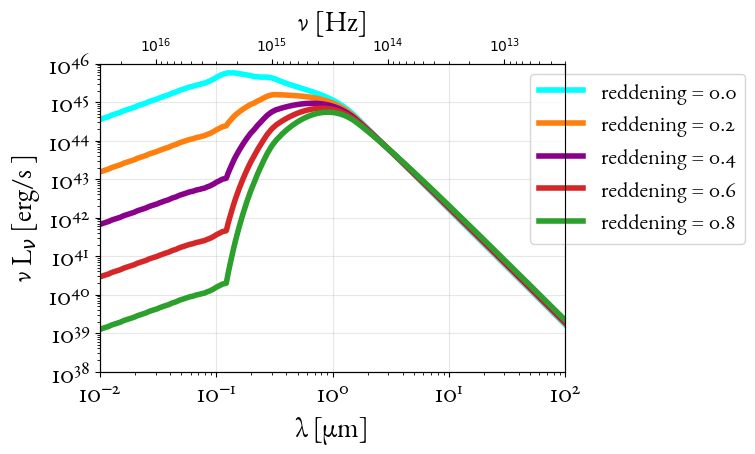
\includegraphics[width = \textwidth]{figures/Templates/BBB_T.png}
 \caption{Accretion disk emission templates by Richards et al. (2006)\cite{Richards2006} for different values of reddening fraction $\mbox{E(B-V)}_{\mbox{\tiny{BBB}}}$. }
  \label{fig:BBB_temp}
\end{figure}
The accretion disk contribution is assumed to be mostly thermal emission from the accretion disk with $T=10^{5 \pm 1} $K, accepting that locally the disk emits like a Black Body, and is parametrised by a reddening fraction (due to absorption from the dusty AGN torus) and a scaling coefficient\cite{Richards2006}. 
The templates are by Richards et al. (2006)\cite{Richards2006} and are shown in Figure \ref{fig:BBB_temp}.\\
The attenuation law due to absorption from the dusty AGN torus follows a curve similar to that of the Small Mangelanic Cloud, as studied on quasars by Hopkins et al. (2004)\cite{Hopkins2004}. Adjacent to equation \ref{eq:dustatten}, the observed flux:
\begin{equation}
     F_{\mbox{\tiny{obs}}}^{\mbox{\tiny{BBB}}}= F_{\mbox{\tiny{intr}}}^{\mbox{\tiny{BBB}}} \times 10^{0.4 A_{\lambda}} 
\end{equation}
and the attenuation law (equations \label{eq:dustatten2} and \label{eq:dustatten3}) is modified accrodingly\cite{Prevot1984}:
\begin{equation}
     \begin{cases}   
     A_\lambda = k_{\mbox{\tiny{BBB}}}(\lambda) \, \mbox{E(B-V)}_{\mbox{\tiny{BBB}}} \\ 
     k_{\mbox{\tiny{BBB}}}(\lambda)  = -0.38+1.39\times(10^{-4} \lambda)^{-1.2}\end{cases}
\end{equation}
The Accretion disk models, have two free parametres: the reddening fraction, and a scaling factor that measures the accretion disk's amplitude (shown in Table \ref{tab:ParamSpace}).
%-------------------------------------------------------------------------------%
%-------------------------------------------------------------------------------%
%-------------------------------------------------------------------------------%
%-------------------------------------------------------------------------------%
%-------------------------------------------------------------------------------%

\section{AGN Torus} \label{sec:SED/AGNtorus}
%https://academic.oup.com/mnras/article/355/3/973/954352#91918618
In a galaxy hosting an active galactic nucleus, the AGN dust torus heated by the hard radiation from the accretion disk (which, in turn, is accreting onto a supermassive black hole) emits thermal radiation that contributes to the mid-infrared (MIR) spectral band and might, even, dominate the MIR emission over that produced by the diffuse dust and stellar component for luminous AGNs. The toroidal structure and dust composition stems from the unification model\cite{Antonucci1993}.\\
The intense radiation emitted by the disk, due to the internal friction of the gas, is then absorbed by this dust which is heated to the highest possible temperatures (around 1000-1500 K) and is then re-emitted as thermal radiation in the 2-40 μm domain\cite{Fritz2006}.
The AGN torus is a dust stucture\cite{GarciaGonzalez2017} and dynamical studies tend to favour\cite{Elitzur2006} a clumpy structure rather than a uniform torus (with dust "clumps" or clouds as shown in Figure \ref{fig:CAT3D}). \\
%Assuming a dust-cloud distribution $\eta (r, \theta)$, where $r$ is the radial coordinate and $\theta$ the altitude coordinate angle, $\eta$ is  the normalized number of clouds per unit length, so that $$ N_0 \,\eta(r, \theta) = \pi\, R_{\mbox{\tiny{cloud}}}^2 \, \rho_N $$
%where $\rho_N$ is the cloud number density per unit volume. The volume filling factor $Φ_V$ can be calculated by multiplying the cloud number density per unit volume $\rho_N$ with the cloud volume $V_{\mbox{\tiny{cloud}}} = 4\pi R_{\mbox{\tiny{cloud}}}^3/3$, resulting to $$  Φ_V = \dfrac{4}{3} N_0\, \eta(r, \theta)\, R_{\mbox{\tiny{cloud}}}$$
%H{\"o}nig \& Kishimoto (2010)\cite{HonigKishi2010} show that a surface filling factor $σ_s (r)$ can be described using cloud number density $ \rho_N $ projected in the vertical z-direction of the cylindrical coordinate
%\begin{equation}
%    σ_s (r) = \int_{-\infty}^{\infty}\; \pi R_{\mbox{\tiny{cloud}}}^2 \,\rho_N\,dz
%\end{equation}
%with the explicit dependence $σ_s (r) \propto r^{\alpha_{\mbox{\tiny{clouds}}}}$. 
Assuming a dust-cloud distribution where $r$ is the radial coordinate, H{\"o}nig \& Kishimoto (2010)\cite{HonigKishi2010} assert that a surface filling factor $σ_s (r)$ can be described by the dependence 
\begin{equation}
    σ_s (r) \propto r^{\alpha_{\mbox{\tiny{clouds}}}}
\end{equation}
Consequently, the luminosity is calculated by multiplying the surface filling factor with the source function of the clouds $S_\nu(r) $ and integrating from the inner radius (sublimation radius) to the outer radius of the torus: 
\begin{equation}
   L_\nu^{\mbox{\tiny{Torus}}} = 2\pi \int_{r_{\mbox{\tiny{sub}}}}^{R_{\mbox{\tiny{out}}}}\;  σ_s (r) \, S_\nu(r)\,r \, dr
\end{equation}

\subsection{Torus model \textit{\&} parameters}
As explained above (Section \ref{sec:SEDmodelling}, the dusty torus is the essential component to explain the orientation dependence on the unified model. There are some constraints for the torus that can be inferred from indirect evidence. A large number of torus models have been presented in the literature to explain the IR observations.\\
The \code{CAT3D}\footnote{\url{cat3d.sungrazer.org}} software, described in detail by H{\"o}nig \& Kishimoto (2010)\cite{HonigKishi2010}, has been run by Markos Polkas to produce AGN torus templates which are scaled for each galaxy and used in the present thesis. These are radiative transfer models of three-dimensional clumpy dust tori using optically thick dust clouds and a low torus volume filling factor, and represent the accretion disk-powered infrared luminosity.\\
The diffuse radiation field in the torus is approximated by a statistical approach and there are three dust compositions and grain sizes: the standard ISM (47\% graphites and 53\% silicates), ISM large grains (grains between 0.1 and 1 μm in size), and Gr-dominated (dominated by intermediate to larger graphite grains, 70\% graphites and 30\% silicates). \\
The parameters of this library of SEDs are (schematically depicted in Figure \ref{fig:CAT3D}):  
\begin{itemize}
    \item The viewing angle $i$
    \item The number of clouds along an equatorial line-of-sight $N_0$
    \item The radial dust-cloud distribution power-law index $\alpha_{\mbox{\tiny{clouds}}}$
    \item The half-opening angle of the distribution of clouds $\theta_0$
\end{itemize}
An additional parametre, as already noted, is a scaling factor that adjusts the SED amplitude for each galaxy. The optical depth $\tau_{\mbox{\tiny{clouds}}}$ of the individual clouds and the outer torus radius $R_{\mbox{\tiny{out}}}$ in units of the sublimation radius $r_{\mbox{\tiny{sub}}}$ are used in the \code{CAT3D} code to produce the SED templates. The sublimation radius forms the inner boundary of the dust distribution (inner torus radius) where the dust becomes too hot to survive. 
This library includes model SEDs in the $0.01-36000 \,$μm wavelength range.
Some indicative templates are plotted in Figure \ref{fig:Torus_temp}.
%These models are characterized by six parameters that have direct influence on the IR dust SEDs of AGN. These are: (1) the power-law index of the radial dust-cloud distribution a, that is ∝ra; (2) the half-covering angle of the torus θ0; (3) the number of clouds along an equatorial line-of-sight N0; (4) the torus outer radius Rout; (5) the optical depth of the individual clouds τV; and (6) the inclination(i.e. the viewing angle) i. In Fig. 5, we show a sketch of some of the CAT3D torus model parameters. The AGN is assumed to be radiating in an isotropic manner. \cite{GarciaGonzalez2017}
\begin{figure}
\centering
  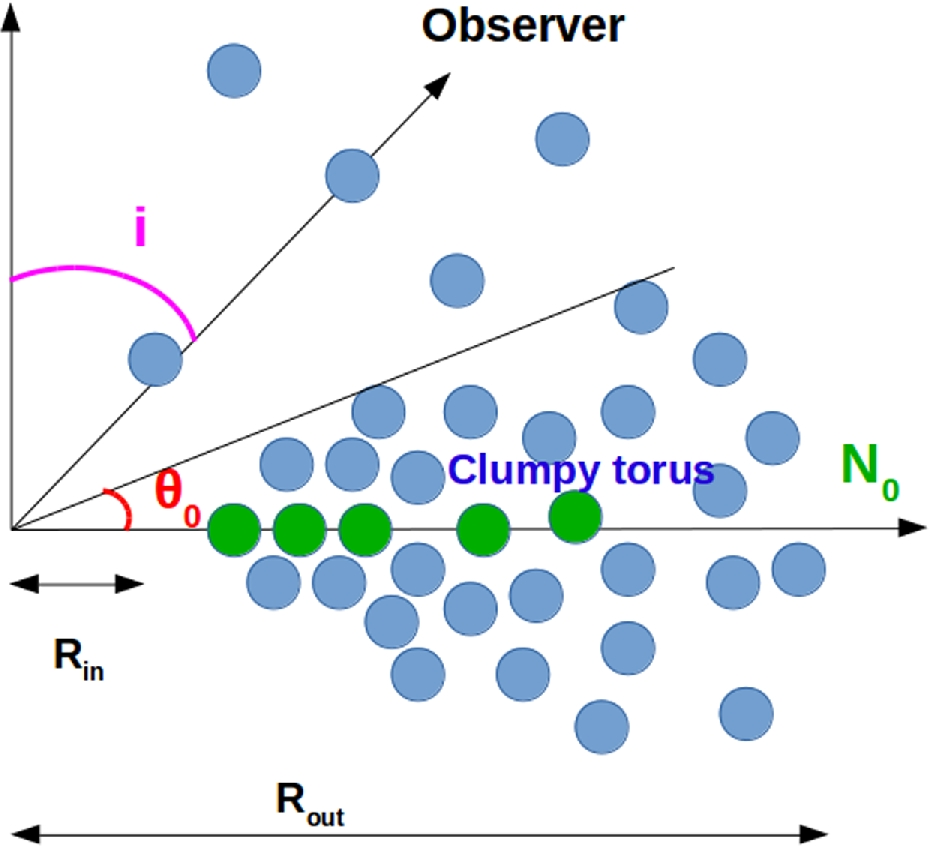
\includegraphics[width = 0.6\textwidth]{figures/TORUSparams_Cat3d.jpeg}
 \caption{AGN clumpy torus cartoon plot. The origin represents the SMBH, the horizontal axis represents the plane of the torus, $R_{\mbox{\tiny{in}}}$ and $R_{\mbox{\tiny{out}}}$ are the inner and outer radius of the torus, $R_{\mbox{\tiny{in}}}$ is essentially the sublimation radius. $N_0$ is the number of clouds along an equatorial line-of-sight, $i$ is the inclination of the torus with respect to the observer and $\theta_0$ is the half-angle that covers the torus from the equatorial plane. Image lifted from Garc{\'\i}a-Gonz{\'a}lez et al. (2017)\cite{GarciaGonzalez2017} }
  \label{fig:CAT3D}
\end{figure}
\begin{figure}
\centering
  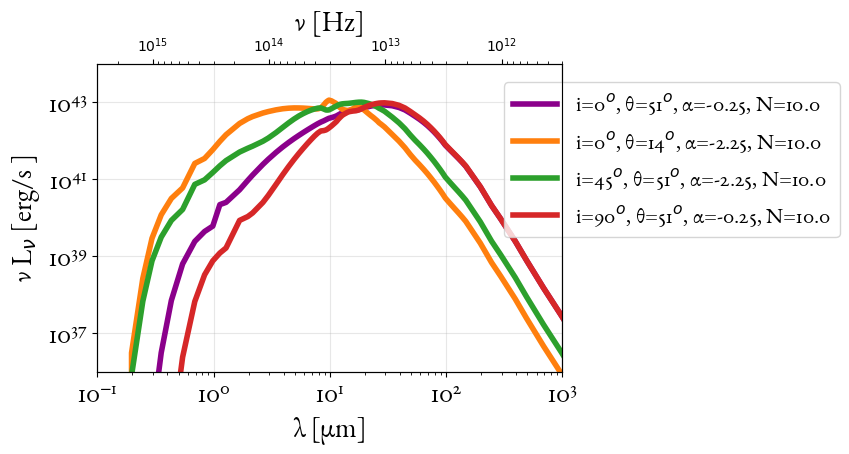
\includegraphics[width = \textwidth]{figures/Templates/Torus_T.png}
 \caption{AGN torus emission templates generated by Markos Polkas using \code{CAT3D}\cite{HonigKishi2010}. Here plotted some indicative values of viewing angle $i$, half-covering angle of torus $\theta$, spectar index of dust-cloud distribution $\alpha$ and number of clouds along an equatorial line-of-sight $N$, with the same amplitude scaling. }
  \label{fig:Torus_temp}
\end{figure}

%\cite{GarciaGonzalez2017}
%\subsection{Dust extinction and attenuation}
%https://dust-attenuation.readthedocs.io/en/latest/dust_attenuation/model_flavors.html#charlot-fall
%https://arxiv.org/pdf/2001.03181.pdf
%https://ned.ipac.caltech.edu/level5/Sept12/Calzetti/Calzetti1_4.html
%https://www.aanda.org/articles/aa/full_html/2018/11/aa33841-18/aa33841-18.html
%https://iopscience.iop.org/article/10.1086/309250/meta
%https://iopscience.iop.org/article/10.1086/309250/pdf
%https://iopscience.iop.org/article/10.3847/1538-4357/aaed25/pdf
%https://dust-extinction.readthedocs.io/en/stable/?fbclid=IwAR1iM4ed9UsoQDP8BdpQ_H_7nAr3JpF-X6uN8f_i98VneiW1PG4pylBgZwA
%https://dust-extinction.readthedocs.io/en/stable/dust_extinction/model_flavors.html#average-models
%https://ui.adsabs.harvard.edu/abs/2011ApJ...737..103S/abstract

\section{Synchrotron radio emission}\label{sec:SED/radio}
At radio frequencies the emission is split between:
\begin{itemize}
    \item Thermal processes: related to the ionisation of the gas by massive stars
    \item Non-thermal processes: related to the interaction of relativistic electrons from supernovae with local magnetic fields and free-free emission from HII regions, also synchrotron emission related to the supermassive black hole.
\end{itemize}

\subsection{Radio jet model \textit{\&} parametres}
The exact shape and intensity of the synchrotron spectrum depends on various parameters such as the strength of the magnetic field, the energy of the relativistic electrons propagating through it. Rather than attempting to model the synchrotron in such detail, the synchrotron component of the present code relies on a single power-law spectral slope with cutoff and on the assumption that between frequencies $10^8\,\mbox{Hz}$ and $3\times 10^{10}\,\mbox{Hz}$ the spectrum is largely dominated by non-thermal (synchrotron) emission, which is ensured by design in the ARC survey. The specific flux for the radio component is: 
\begin{equation}
    f_{\nu}^{\mbox{\tiny{rad}}} = A_{\mbox{\tiny{rad}}}\times \Big( \dfrac{\nu}{10^9 \mbox{Hz}} \Big)^{\alpha_{\mbox{\tiny{rad}}}} \times e^{-\nu/\nu_{\text{\tiny{cutoff}}}} 
    \label{eq:radio}
\end{equation}
The model for the radio component of the SED is the analytic function of equation \ref{eq:radio}, where $\nu_{\text{\tiny{cutoff}}} = 10^{12}$ Hz,  and the parametres are the spectral index $\alpha_{\mbox{\tiny{rad}}}$ and the scaling factor $A_{\mbox{\tiny{rad}}}$.

%https://iopscience.iop.org/article/10.3847/0004-637X/827/2/109
%https://ned.ipac.caltech.edu/level5/Condon/condon4_1.html
% https://www.aanda.org/articles/aa/full_html/2018/03/aa31673-17/aa31673-17.html
%a mean slope αnth = 0.59 ± 0.20 in the low-frequency regime, and a break or an exponential decline in the frequency range of 1–12 GHz
%FIR–RADIO CORRELATION  %https://iopscience.iop.org/article/10.3847/0004-637X/827/2/109


\section{Other Components}\label{sec:blazar}
In order to construct an astrophysically sound spectral model for a galaxy, a nebular emission can be modelled (e.g. with photoionisation modeling such as the code \code{CLOUDY}\cite{CLOUDY}). Since nebular emission does not contribute significantly to the continuum and only adds the spectral emission line features, in the present work it is omitted from the photometric SED models.\\
A more complete model that can encompass different types of galaxies, could benefit from additional components, such as blazar emission model, hot corona X-ray emission, intergalactic medium (IGM), Lyman-α forest (LAF), Damped Lyman alpha (DLA) modeling and extend to joint models of morphology and SED. \\
Since the ARC survey contains many blazars, in the future, a model component for the blazar sequence ought to fortify and extend the SED modelling.

%IGM (LymanAlphaForest/Damped” Lyman alpha (DLA) modeling)
%hot corona emission
%blazar sequence
%--------------
%future: 
%SSPs DSPS, emulators
%SFHs nonparametric
%Dust radiative transfer, simulations, ML
%Lya modeling
%Metallicity histories
%joint models of morphology and SED

\section{Model photometry}\label{sec:filters}
In order to model the observed photometry, the models described above can be projected into the data space with filter projections. 
In photometry, a filter band describes the response of the astronomical observation (composed of the atmosphere, telescope, instrument, and detector) to the light from the source. Therefore, it encapsulates the actual spectral information inherent in the corresponding photometry from the SED.
The average flux through a filter band (and consequently the one used to calculate rest-frame luminosity of each SED data point) is
\begin{equation}
    <F>_b = \dfrac{ \int \; R_\gamma^b\; f_\nu \;d \nu }{\int \; (\nu/\nu_b)^\beta \; R_\gamma^b \;d \nu }
\end{equation}
where $b$ denotes the band pass corresponding to the selected filter, $f_\nu $ is the observed flux, $R_\gamma^b$ is the relative response of the filter $b$ per photon ($\gamma$). The factor $(\nu/\nu_b)$ in the denominator is for calibration purposes, for UV, optical and near-IR $\beta = 0$, while for IR photometry $\beta = 1$ and some far-IR instruments adopt $\beta = 2$.\\
The transmission profiles $R_\gamma^b (\nu)$ (usually in units of relative response per photon) of many surveys' filters can be found at \url{http://svo2.cab.inta-csic.es/svo/theory/fps/}.\\
The aforementioned service couldn't provide the transmission curves for all band passes of the ARC SEDs, thus, in the present work, no filters were used, assuming  $<F>_b \approx f_{<\nu>_b} <\nu>_b$, where $<\nu>_b$ is the dominant frequency of filter band $b$, effectively assuming monochromatic energy of the radiation for each SED point. In the future, a more diligent search for transmission curves and the corresponding application of those curves on the modelled SEDs would provide a more robust model photometry.   




